\documentclass[../Aurora C# unofficial manual.tex]{subfiles}

\begin{document}
	\section{Modifying stars}\label{1_modifying_stars}
	Original post can be found
	\href{http://aurora2.pentarch.org/index.php?topic=8495.msg118725#msg118725}{here}.
	\newline\newline
	
	C\# Aurora allows you to manipulate star systems in SM Mode. While it would be difficult to design a system during the original generation process, due to the complexities involved, you can now add or modify stars and system bodies. This post covers modifying stars.
	
	You click on a star in the System View and then click Change Star. The dialog below pops up and allows you to select spectral class, orbital distance, bearing and parent star.
	\begin{figure}[h]
		\centering
		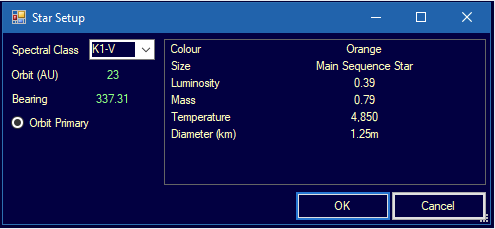
\includegraphics[width=0.5\linewidth]{images/StarSetup}
		\caption[Star Setup]{Star Setup}
		\label{fig:starsetup}
	\end{figure}
	Here is an example from my current test campaign that changes the B component of Alpha Centauri from a K1-V star to an F0-V, which is much hotter. The star will orbit more quickly due to the increased mass, plus all the planets orbiting the star are affected by the increased mass and luminosity of the different star. Temperatures will change, along with potentially hydrosphere type and atmospheric composition (as gases freeze out or boil). Oceans or ice sheets may convert entirely to water vapour given a significant temperature rise. Planets may change their tide-locked status.
	\begin{figure}[H]
		\centering
		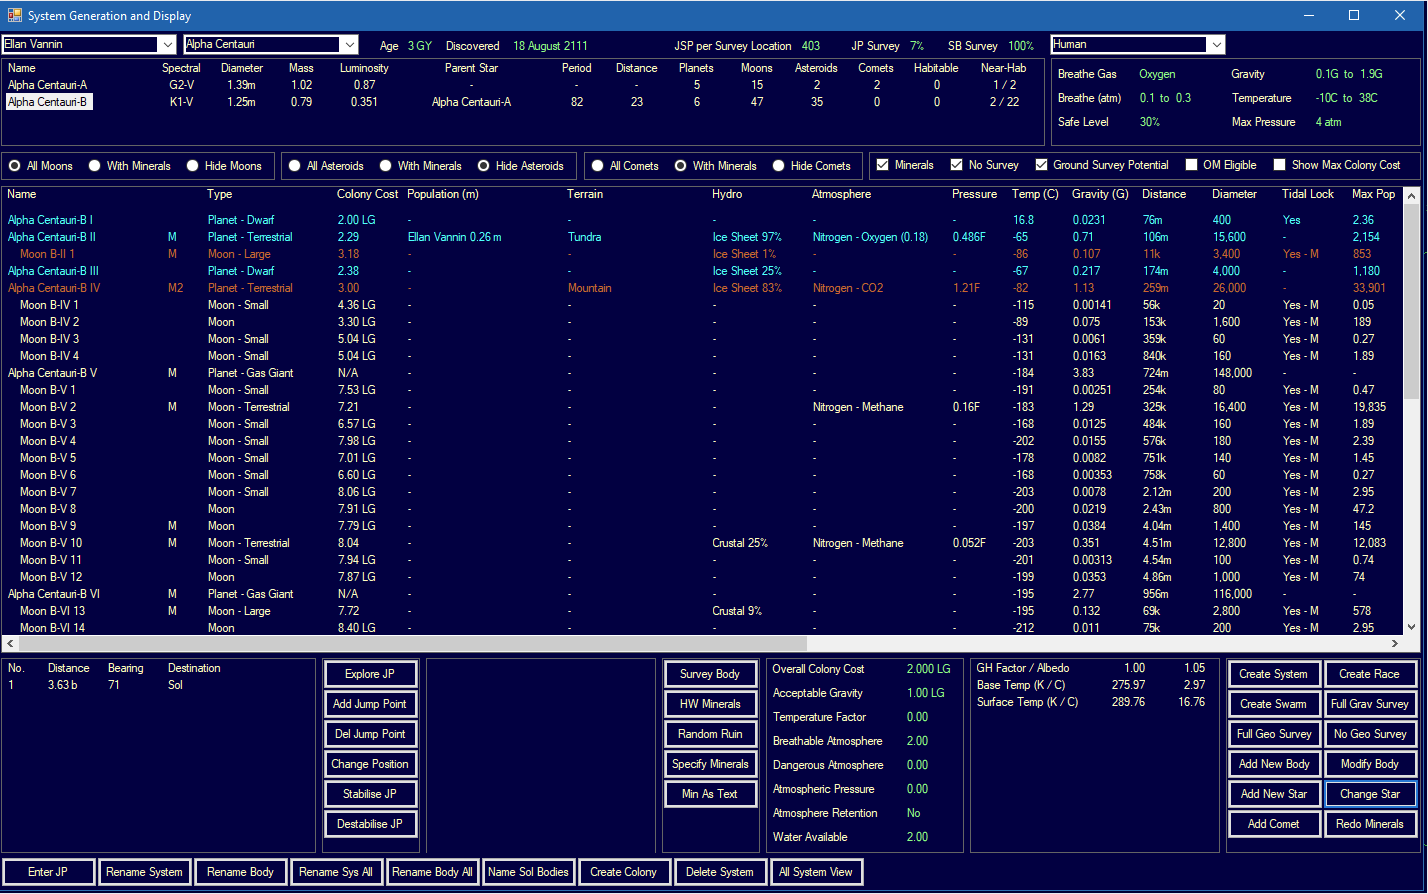
\includegraphics[width=0.95\linewidth]{images/StarSetupExample}
		\caption[Star Setup Example]{Star Setup Example 1}
		\label{fig:starsetupexample}
	\end{figure}
	\begin{figure}[H]
		\centering
		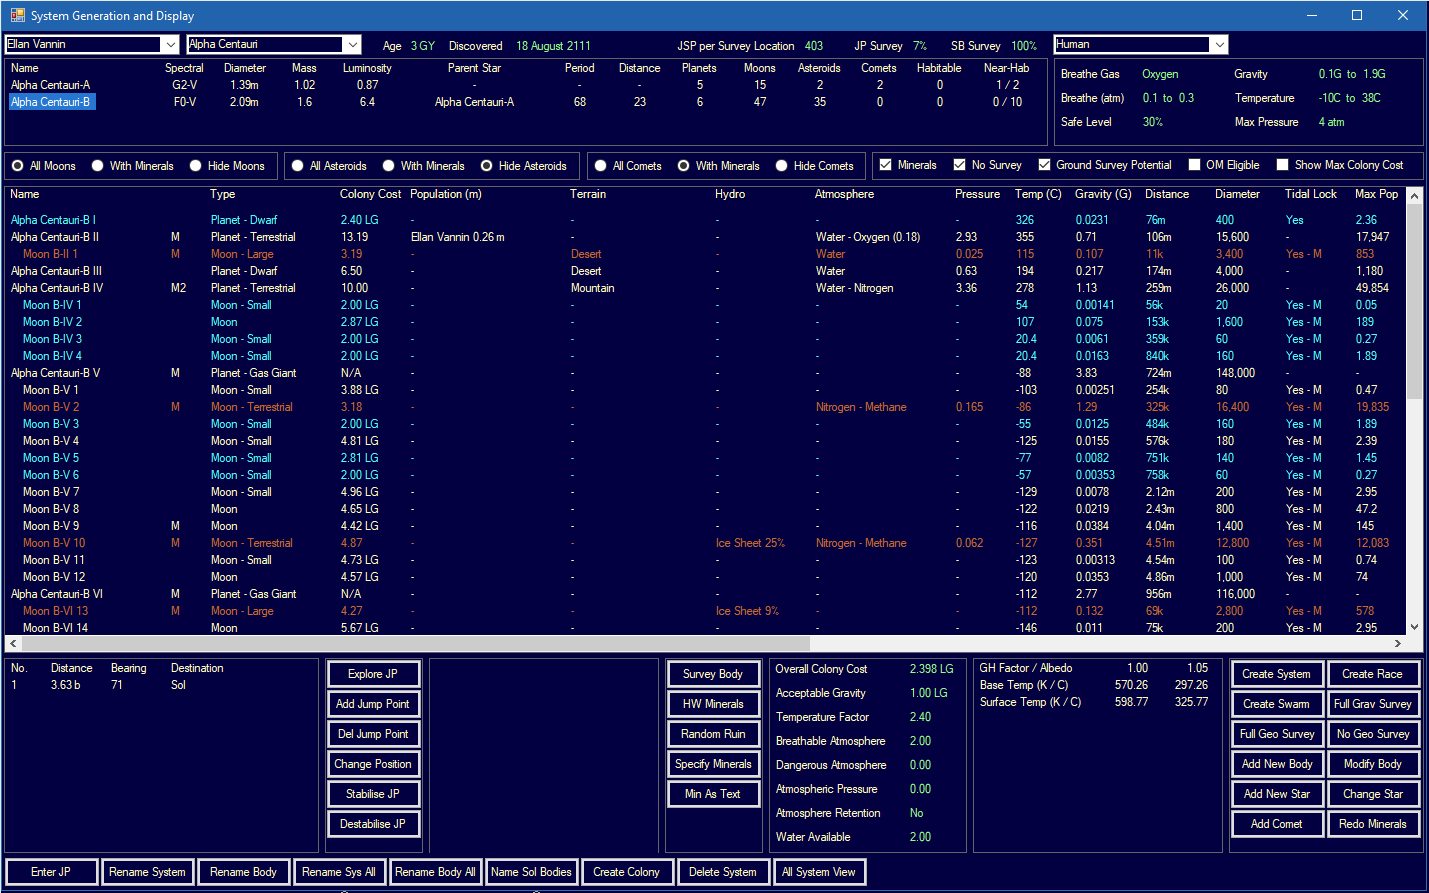
\includegraphics[width=0.95\linewidth]{images/StarSetupExample2}
		\caption[Star Setup Example 2]{Star Setup Example 2}
		\label{fig:starsetupexample2}
	\end{figure}

	These two screenshots show the effect of moving the star further from the primary.
	\begin{figure}[H]
		\centering
		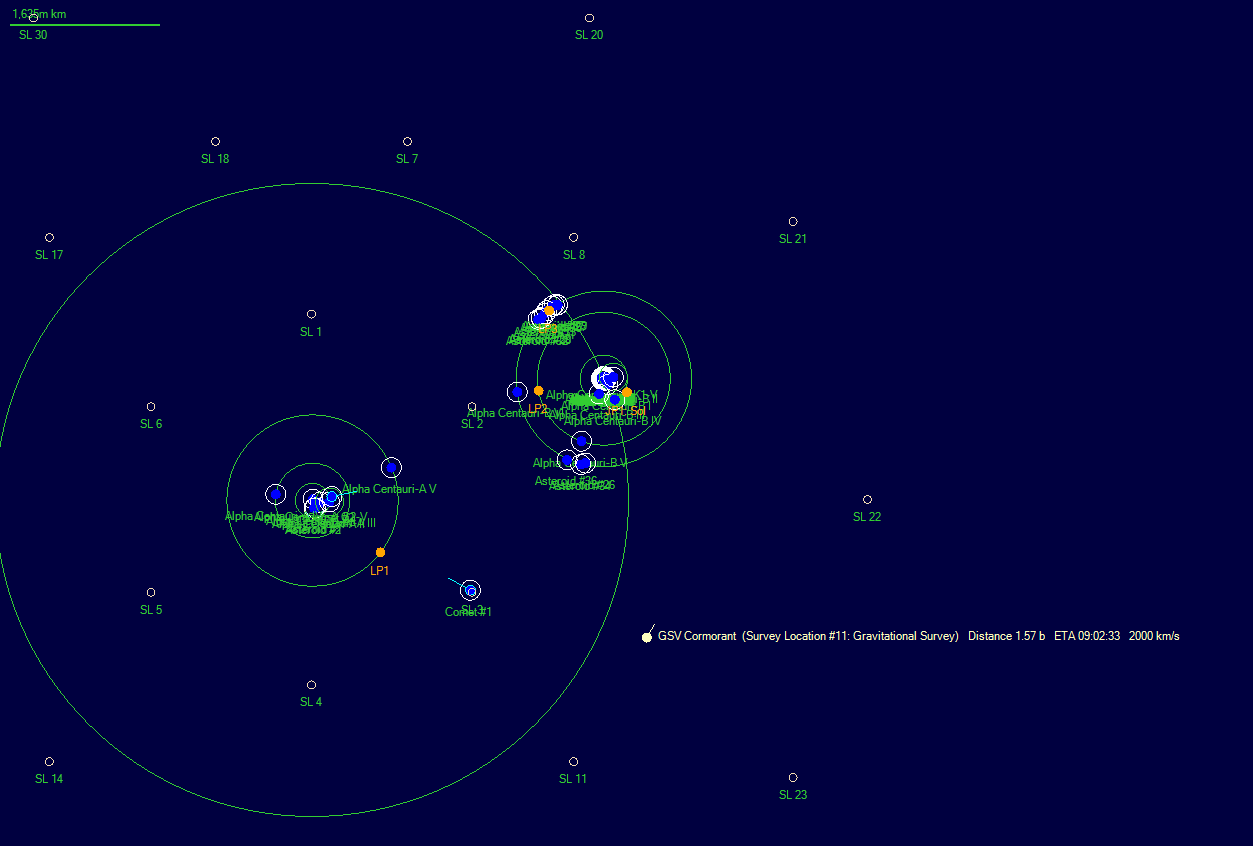
\includegraphics[width=0.95\linewidth]{images/Engineering003}
		\caption[Engineering Example]{Engineering Example 1}
		\label{fig:engineering003}
	\end{figure}
	\begin{figure}[H]
		\centering
		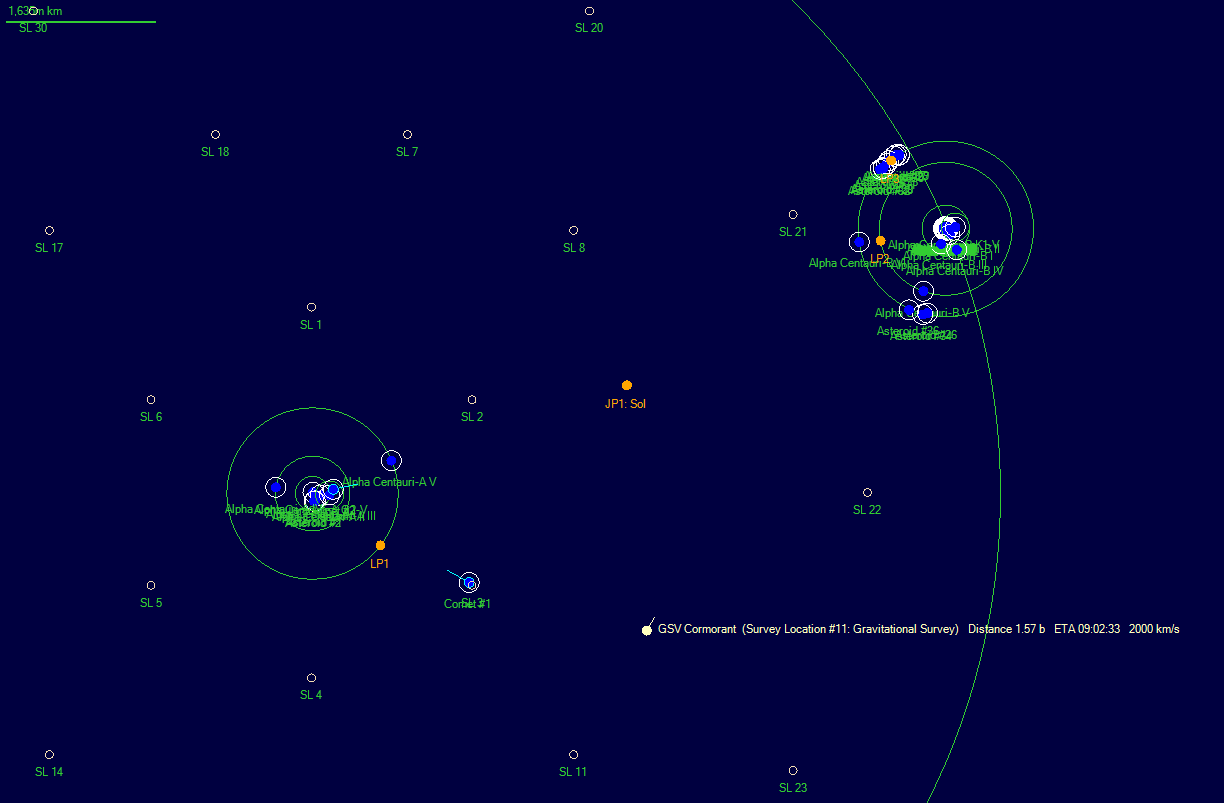
\includegraphics[width=0.95\linewidth]{images/Engineering004}
		\caption[Engineering Example 2]{Engineering Example 2}
		\label{fig:engineering004}
	\end{figure}
	
	
	\section{Adding stars}\label{2_adding_stars}
	Original post can be found
	\href{http://aurora2.pentarch.org/index.php?topic=8495.msg118727#msg118727}{here}.
	\newline\newline
	
	Adding a new star is straightforward. You click Add New Star. The dialog below pops up and allows you to select spectral class, orbital distance, bearing and parent star.
	\begin{figure}[H]
		\centering
		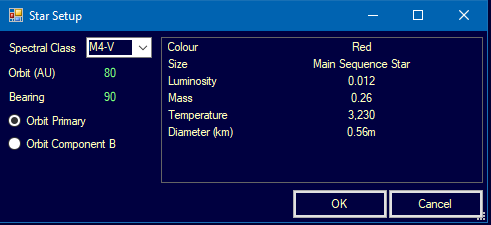
\includegraphics[width=0.5\linewidth]{images/AddingStar}
		\caption[Adding Star]{Adding Star}
		\label{fig:addingstar}
	\end{figure}
	
	This screenshot shows the result of adding the above star to the Alpha Centauri system. New stars do not have any planets or other system bodies. These are added separately and will be covered in a future post.
	\begin{figure}[H]
		\centering
		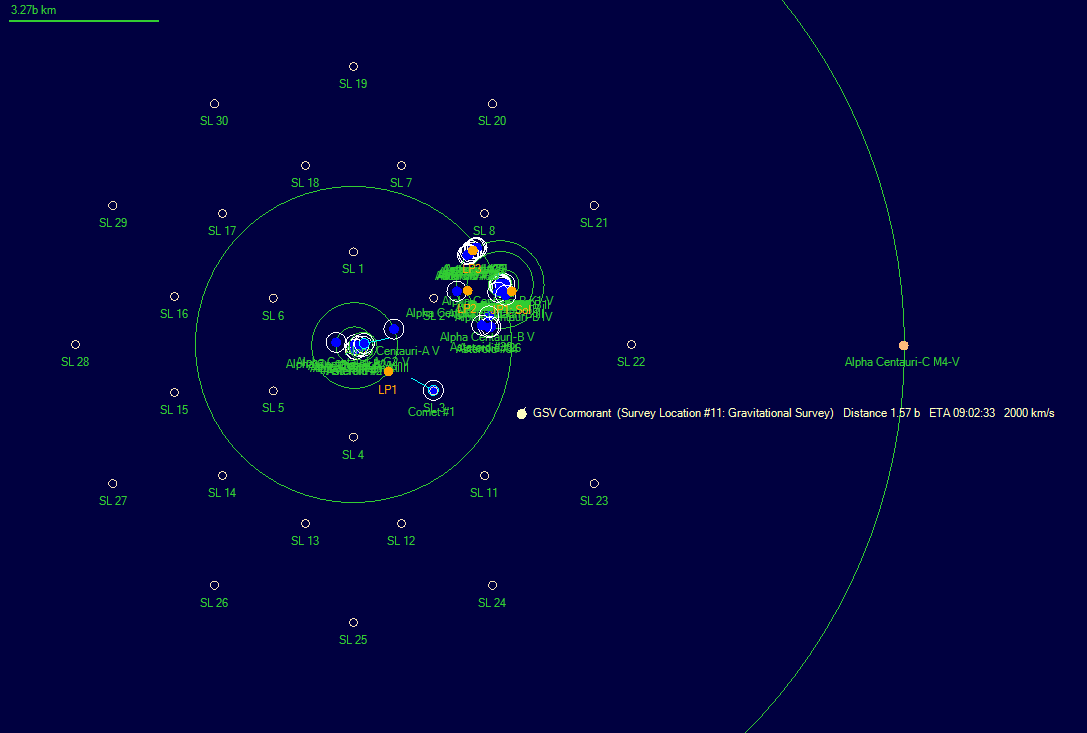
\includegraphics[width=0.95\linewidth]{images/AddingStar2}
		\caption[Adding Star Result]{Adding Star Result}
		\label{fig:addingstar2}
	\end{figure}
	

	\section{Modifying system bodies}\label{3_modifying system_bodies}
	Original post can be found
	\href{http://aurora2.pentarch.org/index.php?topic=8495.msg118744#msg118744}{here}.
	\newline\newline
	
	Modifying system bodies is a more complex process than stars due to the number of factors involved. There are factors that are tied to each other, such as mass, radius, density and gravity, plus certain types of bodies have different rules (planets vs moons, gas giants vs rocky worlds).
	
	Therefore, the following factors can be changed; distance to parent body, diameter, density, hydro extent, albedo, atmospheric composition and dominant terrain. The dominant terrain is restricted to those terrains permitted by the other factors. Factors such as colony cost, gravity, temperature, atmospheric pressure, length of year, maximum population, tidal lock status, atmospheric retention, time required to stabilise a Lagrange point, etc. will all be derived from the factors that can be changed. For example, if you change the diameter or density, the mass and gravity will automatically change. If you change the distance to parent, the temperature and year will change and perhaps the tidal lock status. Finally, factors such as escape velocity, magnetic field, etc. are not shown here because they have no current game play impact, even though escape velocity will change as a result of modifications to density or diameter.
	
	The basic type of system body (terrestrial, dwarf, etc.) cannot be changed, but it will be possible to delete one system body and add a new one of the desired type. This is to ensure all system bodies follow the basic rules of their type, even if they are later modified.
	
	Below is the System Body Modification popup window. You can change the green fields in the top left, the dominant terrain dropdown and can add and remove atmospheric gases by choosing a gas and the desired atm (0 to remove). As you make each change, everything else updates.
	\begin{figure}[H]
		\centering
		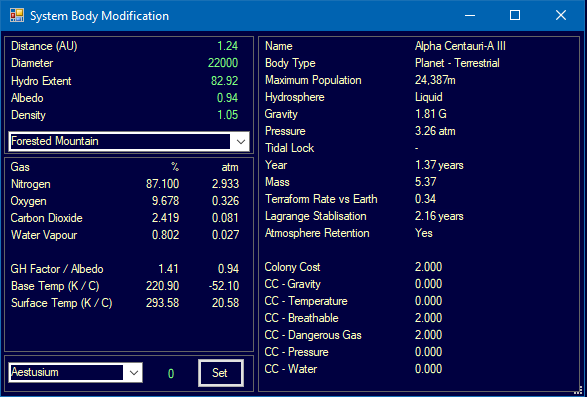
\includegraphics[width=0.5\linewidth]{images/SystemBodyModification}
		\caption[System Body Modification]{System Body Modification}
		\label{fig:systembodymodification}
	\end{figure}
	
	For example, here is what happens if the diameter is halved. Gravity, mass and max population all fall, while the terraform rate vs Earth and the time to stablise a Lagrange point both increase.
	\begin{figure}[H]
		\centering
		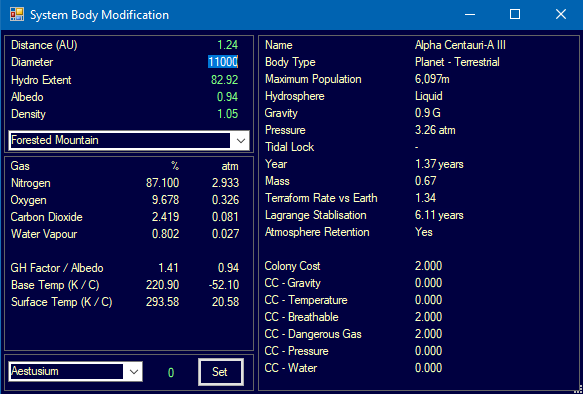
\includegraphics[width=0.5\linewidth]{images/SystemBodyModification2}
		\caption[System Body Modification 2]{System Body Modification Result}
		\label{fig:systembodymodification2}
	\end{figure}
	
	
	\section{Deleting stars and system bodies}\label{4_deleting_stars_and_bodies}
	Original post can be found
	\href{http://aurora2.pentarch.org/index.php?topic=8495.msg118745#msg118745}{here}.
	\newline\newline
	
	Deletion of stars or system bodies is straightforward. Click on the target object and then click Delete Body or Delete Star. You will be given two popup warnings and then the object will be deleted. Deleting a star will remove any system bodies in orbit. Deleting a planet will remove any moons of that planet. Any populations on affected system bodies will be deleted. Deleting the primary star is not possible.
	
	When a star is deleted, any remaining stars will be renamed accordingly. For example, if you delete the B component of a primary, the original C component will now become the B component. When a planet or moon is deleted, the orbit numbers of the planets or moons will be adjusted accordingly.
	
	For example, here are the before and after views of the Alpha Centauri-A system when the fourth planet is deleted.
	\begin{figure}[H]
		\centering
		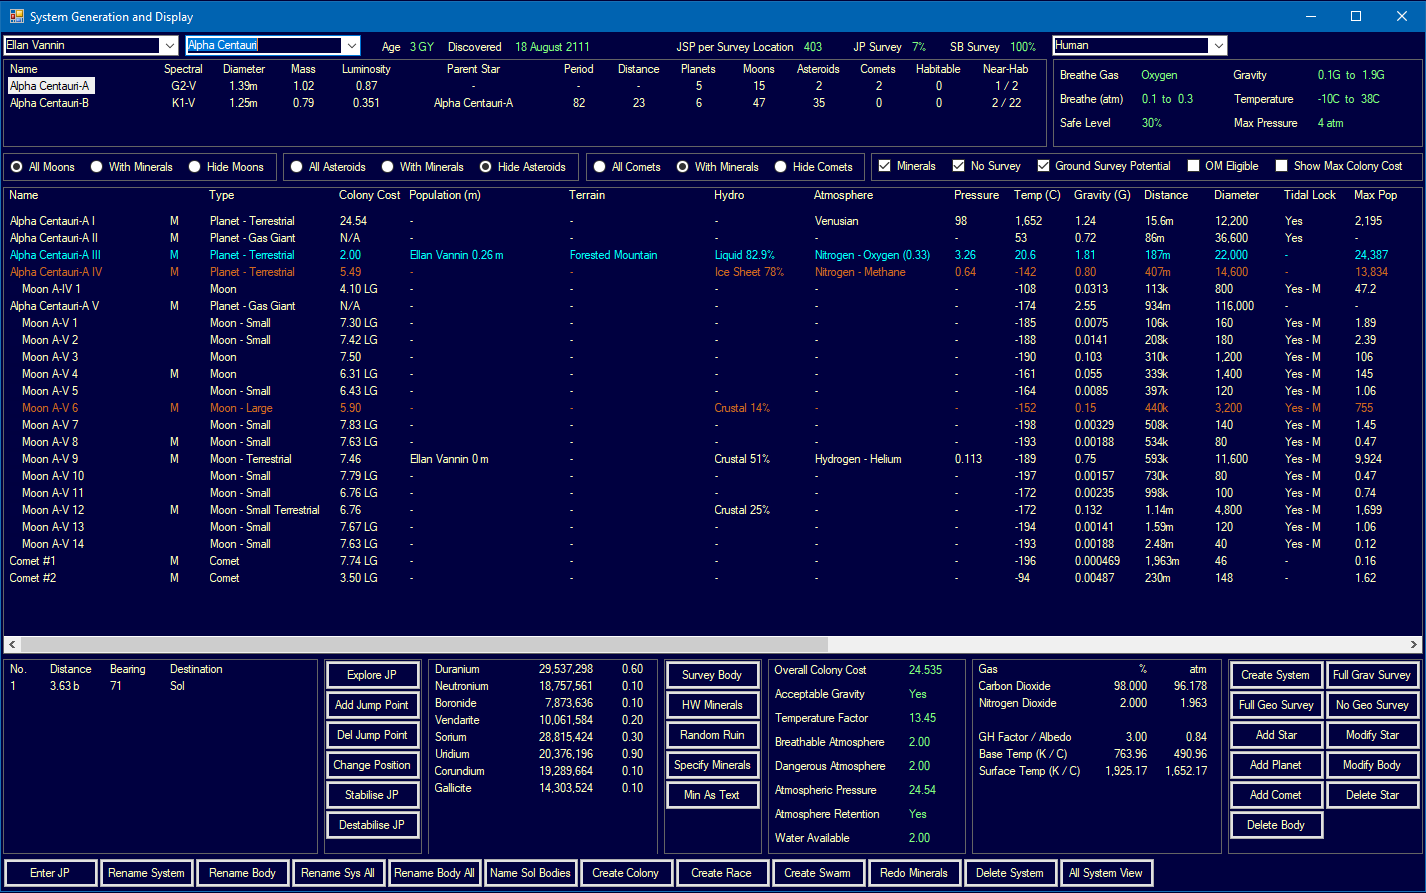
\includegraphics[width=0.95\linewidth]{images/DeletingStarsAndBodies}
		\caption[Deleting Stars And System Bodies]{Deleting Stars And System Bodies}
		\label{fig:deletingstarsandbodies}
	\end{figure}
	\begin{figure}[H]
		\centering
		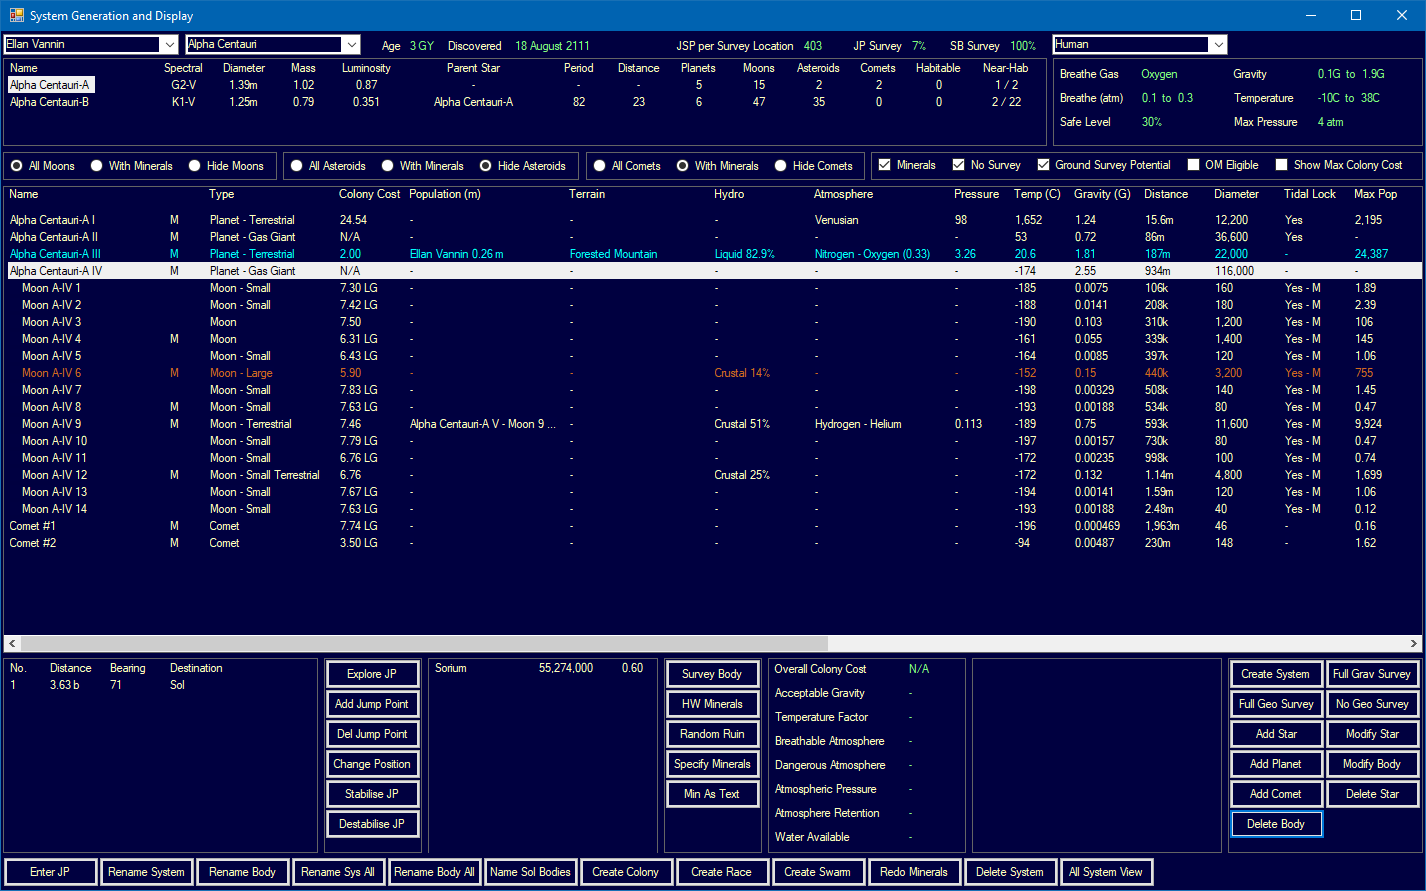
\includegraphics[width=0.95\linewidth]{images/DeletingStarsAndBodies2}
		\caption[Deleting Stars And System Bodies]{Deleting Stars And System Bodies 2}
		\label{fig:deletingstarsandbodies2}
	\end{figure}
	
	\section{Adding planets, comets and asteroid belts}\label{5_adding_planets_comets_asteroid}
	Original post can be found
	\href{http://aurora2.pentarch.org/index.php?topic=8495.msg118767#msg118767}{here}.
	\newline\newline
	
	Below is the form for adding all new system bodies except for additional moons. You choose a system body from the drop down, which includes Terrestrial, Dwarf Planet, Gas Giant, Superjovian, Comet and Asteroid. Each body type has a distance parameter plus one or more other additional options.
	\begin{itemize}
		\item For terrestrial and dwarf planets you have a toggle for automatic moon generation and can choose a specific or random number of moons.
		\item For gas giants and superjovians, you have the above moon options plus similar options for Trojan asteroids (on/off, random/specific).
		\item For comets, you choose the starting distance and maximum distance.
		\item For asteroid belts, you can choose a random or specific number of asteroids and the specific or random width of the belt (how far an asteroid can be generated from the centre of the belt).
	\end{itemize}
	
	Once the planet parameters are selected, press OK and the new body or bodies will appear in the System View. You can select them and use Modify Body to customise if desired.
	
	The various zones shown at the top affect how Aurora determines parameters such as atmosphere, hydrosphere, mineral deposits, albedo, density, number of moons, total mass of asteroid belts and a variety of other factors. There is far too much detail to list, but generally bodies in the life zone will have better conditions and mineral deposits, followed in decreasing order by Inner, Outer and Extreme. These zones also exist in VB6. Of course, those factors only affect initial generation so you can override that by directly modifying a body post-creation.
	\begin{figure}[H]
		\centering
		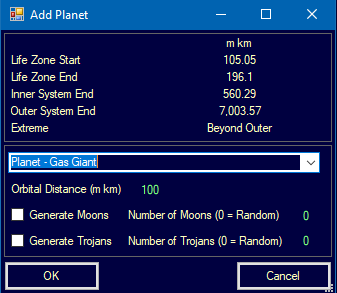
\includegraphics[width=0.5\linewidth]{images/AddPlanet}
		\caption[Add Planet Example]{Add Planet Example}
		\label{fig:addplanet}
	\end{figure}
	
	
	\section{Adding moons and Lagrange points}\label{6_adding_moons_and_lagrange}
	Original post can be found
	\href{http://aurora2.pentarch.org/index.php?topic=8495.msg118787#msg118787}{here}.
	\newline\newline
	
	Below is the form for adding moons to existing planets. During planet creation you can specify appropriate moons to be created at the same time using standard moon generation based on the type of planet and is orbital distance. This form, accessed via the Add Moons button, is for creating additional moons which do not have to obey normal size restrictions. The form allows the addition of up to five moons (the drop-downs all start with no moon) with type and distance specified. If more than five moons are needed, the form can be used multiple times for the same parent planet.
	
	After initial generation you can use Modify Body to specify additional detail if required.
	
	The Add Lagrange button adds a Lagrange point to the currently selected body, even if it would not normally qualify for one.
	\begin{figure}[H]
		\centering
		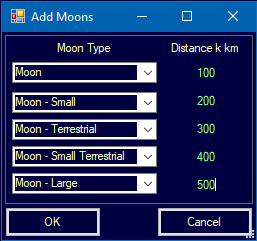
\includegraphics[width=0.5\linewidth]{images/AddMoons}
		\caption[Add Moons Example]{Add Moons Example}
		\label{fig:addmoons}
	\end{figure}
	
	
	\section{Deleting asteroids and Lagrange points}\label{7_deleting asteroids_and_lagrange}
	Original post can be found
	\href{http://aurora2.pentarch.org/index.php?topic=8495.msg118803#msg118803}{here}.
	\newline\newline
	
	Deleting individual asteroids can be done by using the Delete Body button. To delete an entire asteroid belt or all the Trojan asteroids for a particular planet, click one of the asteroids in the belt or one of the Trojans and click Delete Asteroids. There will be two warnings before all the affected asteroids are deleted.
	
	Lagrange Points can be removed by selecting the parent system body and clicking Remove Lagrange.
	
	Below is the final version of the System View in SM mode with all system engineering buttons present.
	\begin{figure}[H]
		\centering
		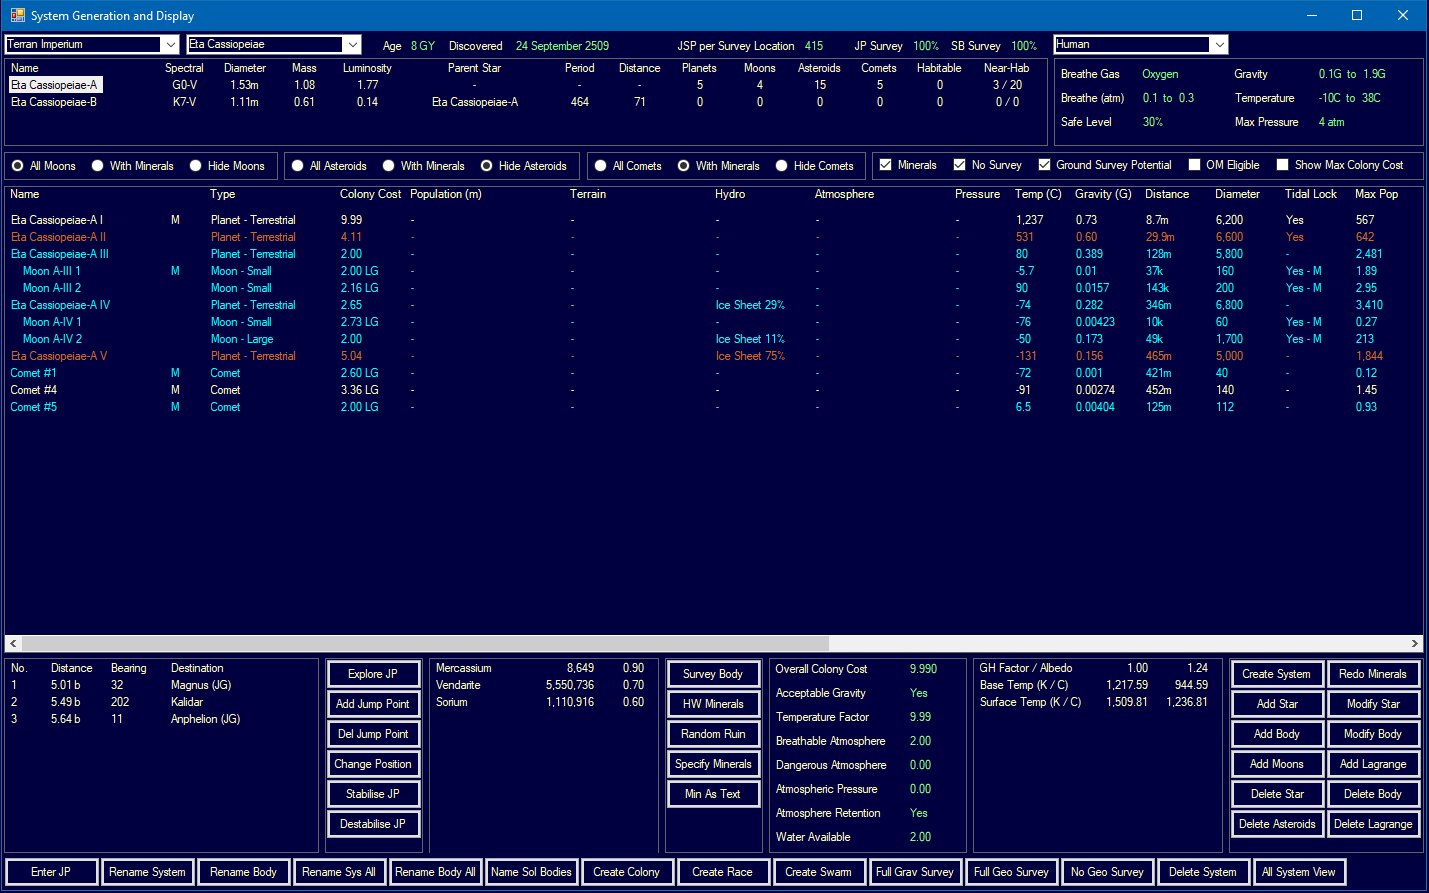
\includegraphics[width=0.95\linewidth]{images/DeletingLagrangePoints}
		\caption[Deleting Lagrange Points]{Deleting Lagrange Points}
		\label{fig:deletinglagrangepoints}
	\end{figure}	
\end{document}